%nearly complete, needs a bit more discussion
\section{Registration}
\label{imp:stitching}
The registration algorithms were implemented in an iterative fashion starting with the simplest. The evolution of ideas has been explained in the design section (Section \ref{design:registration}). \\

\subsection{Input Data}
The input data is a series of point cloud data structures of the person (subject) being scanned. These come from the \emph{person isolation} subsystem. 

\subsection{Initial Issues}
Initial issues with the registration were caused by the coordinate system being inconsistent with the real world. This, along with the fix, will be explained in more detail in Section \ref{impl:point clouds}. A demonstration of this problem can be seen in Figure \ref{fig:wilko poor reg}. \\

\begin{figure}[h!]
    \begin{center}
        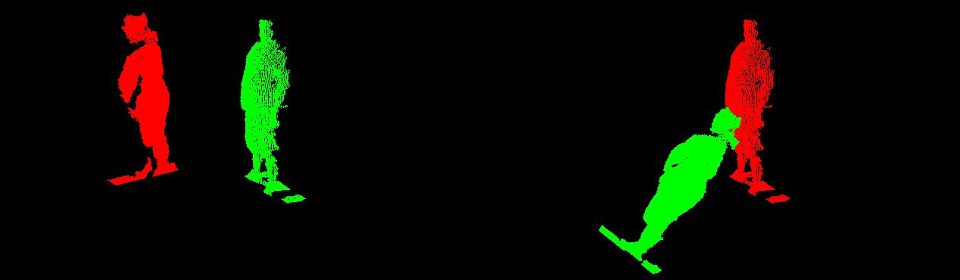
\includegraphics[scale=0.3]{zscreenshots/poor-wilko.jpg}
        \caption{An erroneous registration caused by issues with the coordinate system}
        \label{fig:wilko poor reg}
    \end{center}
\end{figure}

\subsection{Bounding Boxes}
The algorithm was implemented as a class that extends the design pattern stated in Section \ref{design:design pattern}. There were initial problems with alignment due to the bounding boxes on the data scans being artificially increased by parts of the floor that had not been removed during the image acquisition component of the pipeline. This has been demonstrated in Figure \ref{fig:wilko floor problem}. This became known as the \emph{Floor Problem}. Luckily, the floor problem was not intrinsic to the domain and could be mitigated by splitting the image up into a set of planes in $y = 0$ and then removing points in the range of offending planes at the bottom of the image. \\

Once the errors with bounding box were removed a much better registration was achieved, as in Figure \ref{fig:wilko good}. Note that there is still some floor visible which was removed in the iteration which was eventually utilised as the initial alignment for the ICP algorithm. Only two faces have been displayed to make the registration more obvious to the reader. Another dataset, of the Corbett subject, has been used with each scan coloured to demonstrate the overlap. This can be seen in Figure \ref{fig:corbett good}. \\

\begin{figure}[h!]
    \begin{center}
        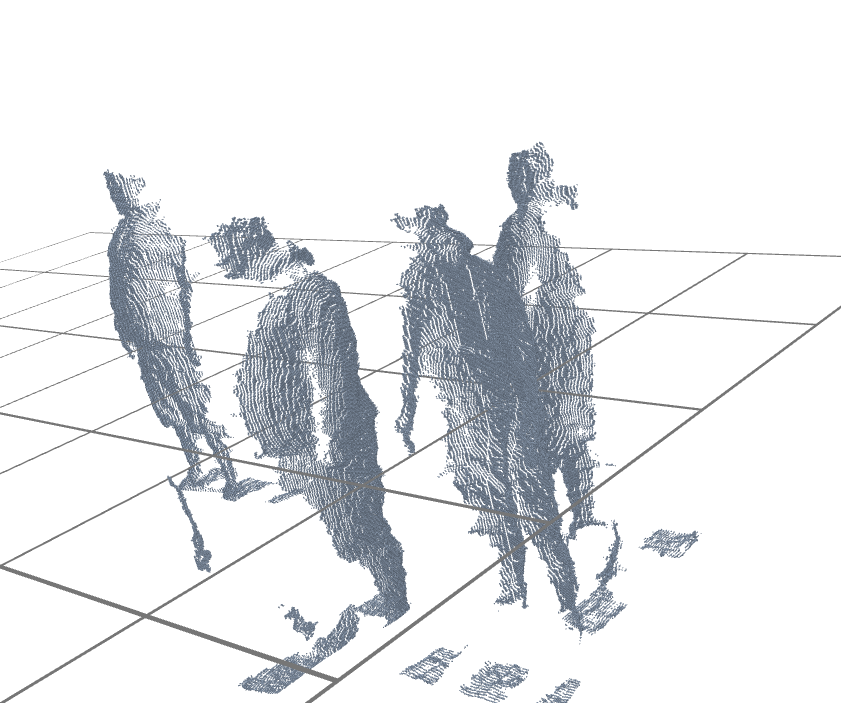
\includegraphics[scale=0.3]{zscreenshots/wilko-floor.png}
        \caption{An erroneous registration caused by issues with the bounding box}
        \label{fig:wilko floor problem}
    \end{center}
\end{figure} \\

\begin{figure}[h!]
    \begin{center}
        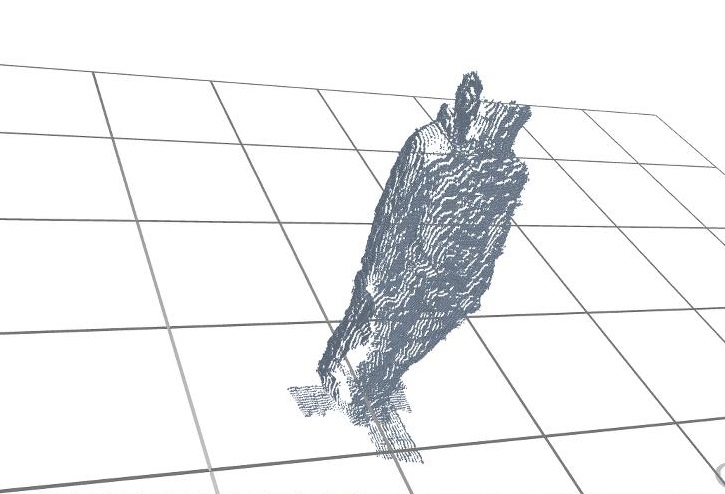
\includegraphics[scale=0.3]{zscreenshots/wilko-good.jpg}
        \caption{A more acceptable registration produced by the bounding box method}
        \label{fig:wilko good}
    \end{center}
\end{figure} \\

\begin{figure}[h!]
    \begin{center}
        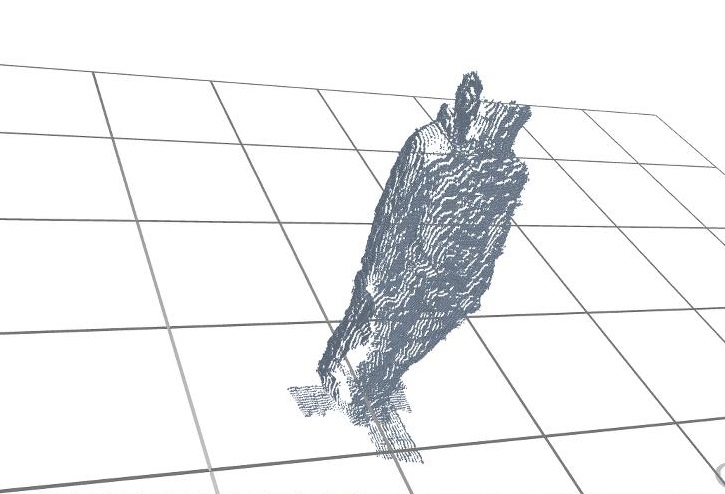
\includegraphics[scale=0.3]{zscreenshots/wilko-good.jpg}
        \caption{The Corbett dataset, registered with the bounding box method and coloured}
        \label{fig:corbett good}
    \end{center}
\end{figure} \\

\subsection{Iterative Closest Points (ICP)}
The ICP algorithm was implemented using the Bounding Box method as the initial alignment. In this case the Corbett dataset has been used again. Figure \ref{fig:corbett icp top} shows a view from above and Figure \ref{fig:corbett icp slant} shows a slanted view from the side. Again the different scans have been coloured to demonstrate the overlap. We can see that there is a much closer correlation between corresponding point pairs than in the initial bounding box method. \\

\begin{figure}[h!]
    \begin{center}
        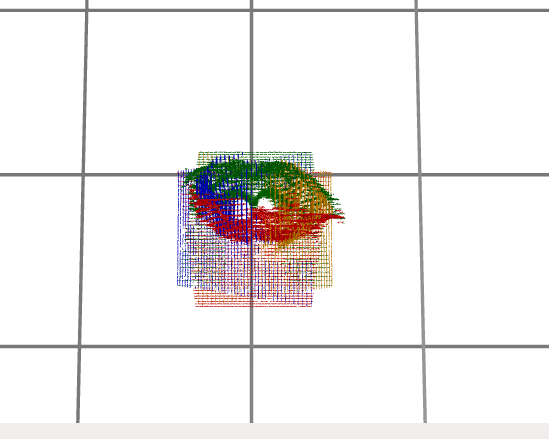
\includegraphics[scale=0.3]{zscreenshots/corbett-icp.png}
        \caption{The Corbett dataset, registered with the ICP algorithm and coloured (birds-eye view)}
        \label{fig:corbett icp top}
    \end{center}
\end{figure} \\

\begin{figure}[h!]
    \begin{center}
        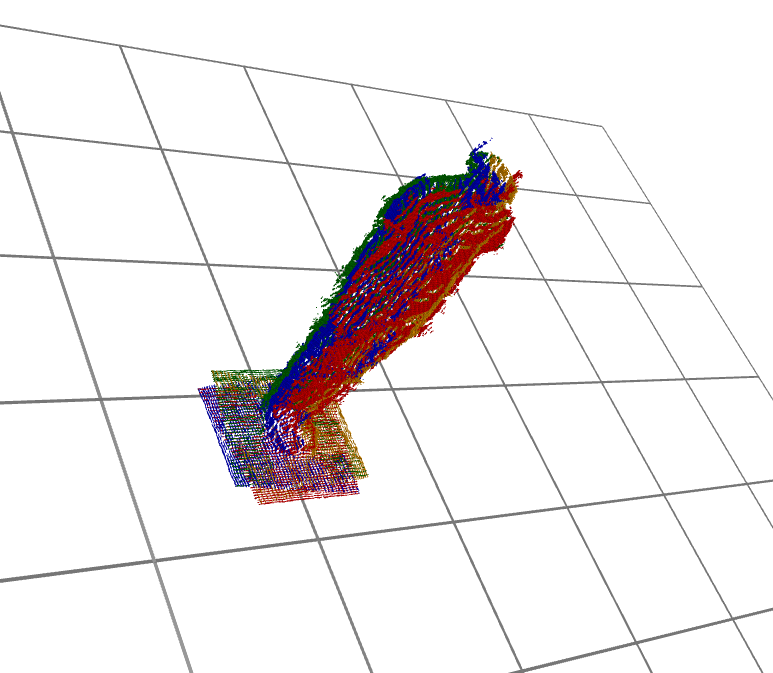
\includegraphics[scale=0.3]{zscreenshots/corbett-icp2.png}
        \caption{The Corbett dataset, registered with the ICP algorithm and coloured (side view)}
        \label{fig:corbett icp slant}
    \end{center}
\end{figure} \\

\subsection{Visualisation}
Visualisation was implemented using the WPF framework, which has been discussed in Section \ref{design:wpf}. Each point in the point cloud is modelled as a very small square which is then input into WPF. This approach is fairly computationally cheap. It could have been made even cheaper by reducing the sample space. This would be achieved by splitting the 3-D coordinate space into a voxel grid and then for every voxel, $\mathcal(V)$ finding the single value, $q$, which is the average of all points $p \in \mathcal(V)$. This is demonstrated in equation \ref{eq:voxel average}. \\

\begin{equation}
    q = \cfrac{\sum{}_i=0^N (p_i_x, p_i_y, p_i_z)}{N}
    \caption{The average of points in a voxel grid}
    \label{eq:voxel average}
\end{equation} \\

A mesh-based approach was attempted but was found to take too much time to render. Considering that the visualisation exists primarily for aesthetic, rather than functional, reasons the mesh approach was ultimately abandoned in favour of the simpler approach. \\ 